% REMEMBER TO SET LANGUAGE!
\documentclass[a4paper,10pt,english]{article}
\usepackage[utf8]{inputenc}
\usepackage[english]{babel}
% Standard stuff
\usepackage{amsmath,graphicx,varioref,verbatim,amsfonts,geometry}
% colors in text
\usepackage[usenames,dvipsnames,svgnames,table]{xcolor}
% Hyper refs
\usepackage[colorlinks=false]{hyperref}

% Document formatting
\setlength{\parindent}{0mm}
\setlength{\parskip}{1.5mm}

%Color scheme for listings
\usepackage{textcomp}
\definecolor{listinggray}{gray}{0.9}
\definecolor{lbcolor}{rgb}{0.9,0.9,0.9}

%Listings configuration
\usepackage{listings}
%Hvis du bruker noe annet enn python, endre det her for å få riktig highlighting.

\lstdefinelanguage{python}
{
	morekeywords={print,abs,for,def,if,while,do,break,return,from,import,try,except,else,elif},
	sensitive=false,
	morecomment=[l]{\#}
}

\lstset{language=python,
	backgroundcolor=\color[rgb]{.95,.95,.95},
	numbers=left,xleftmargin=10pt,
	numberstyle=\tiny,stepnumber=1,numbersep=5pt,
	stringstyle=\color{red},
	basicstyle=\footnotesize \ttfamily,
	keywordstyle=\color{blue},
	commentstyle=\color{green},
	basewidth=0.60em,
	showstringspaces=false,
	captionpos=b,
	frame=single
}

\newcounter{subproject}
\renewcommand{\thesubproject}{\alph{subproject}}
\newenvironment{subproj}{
\begin{description}
\item[\refstepcounter{subproject}(\thesubproject)]
}{\end{description}}

%Lettering instead of numbering in different layers
% \renewcommand{\labelenumi}{\alph{enumi}}
\renewcommand{\thesubsection}{\alph{subsection}}
\renewcommand{\thesection}{\alph{section}}

%opening
\title{FYS-MEK1110 - Mandatory assignment 3}
\author{William Dugan}

\begin{document}

\maketitle

\section{}
We use Pythagoras' theorem:
\begin{align*}
    x = \sqrt{l_0^2-h^2} = 0.4m
\end{align*}

\section{}
As in a., we express the length $l$ in terms of $x$:
\begin{align*}
    l = \sqrt{x^2+h^2}
\end{align*}

\section{}
\begin{figure}[h]
    \centering
    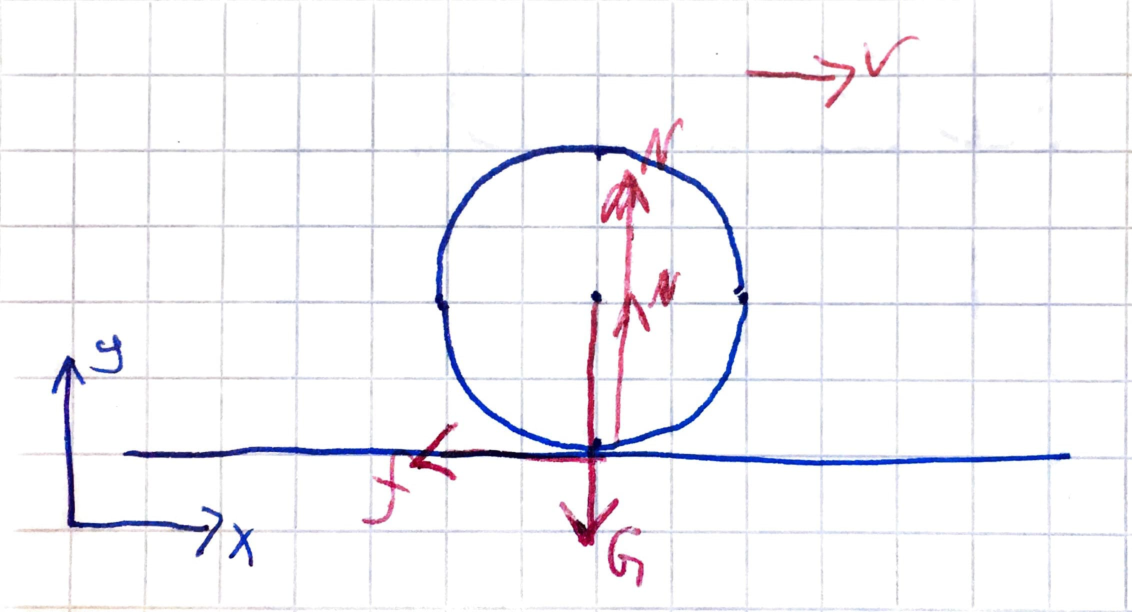
\includegraphics[scale=0.1]{freebodydiagram.JPG}
    \caption{Free body diagram for the cylinder}
    \label{fig:fbd}
\end{figure}
 
\section{}
The spring force is defined as
\begin{align*}
    F_k
    &= -kx \\
    &= -k(l-l_0) \\
    &= -k(\sqrt{x^2+h^2}-l_0) \\
    &= -k \sqrt{x^2+h^2} 
        \left( 
            1 - \frac{l_0}{\sqrt{x^2+h^2}}
        \right)
\end{align*}
The horizontal component of $F_k$ is 
\begin{align*}
    F_x 
    &= F_k\cos\alpha \\
    &= F_k \frac{x}{l} \\
    &= -k x
        \left( 
            1 - \frac{l_0}{\sqrt{x^2+h^2}}
        \right)
\end{align*}
where we have used $l=\sqrt{x^2+h^2}$.

\section{}
\lstinputlisting{oppgave_e.py}

\newpage
\begin{figure}[h]
    \centering
    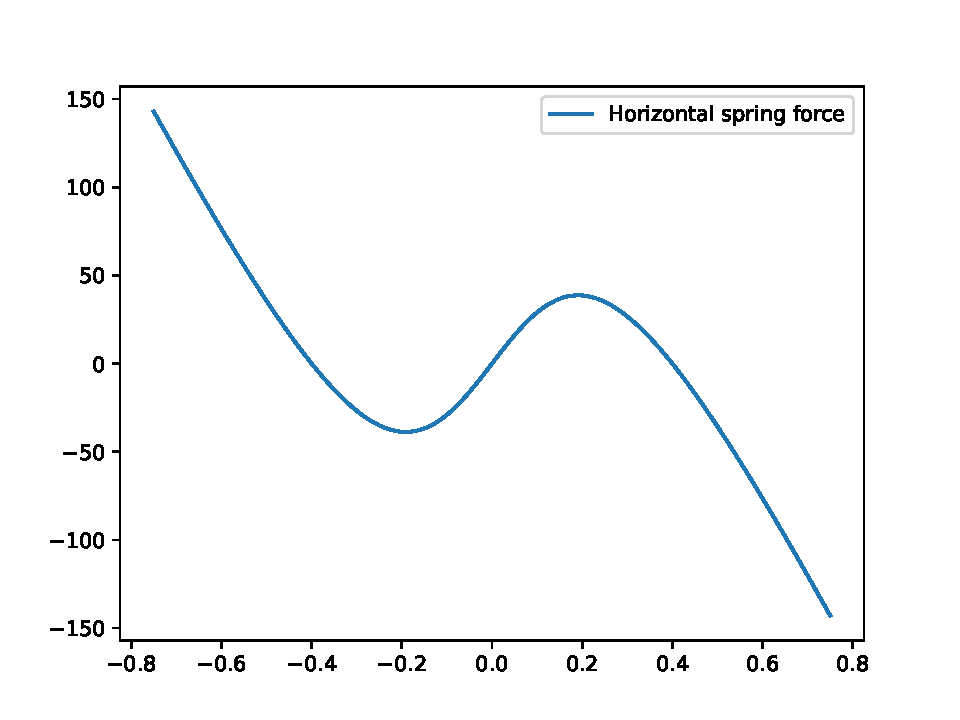
\includegraphics[scale=0.85]{figure_e.pdf}
    \caption{Horizontal component of spring force for $x\in[-0.75, 0.75]$.}
    \label{fig:oppgave_e}
\end{figure}
We observe that the force, and therefore the acceleration, is proportional to and in opposite direction of the movement. This tells us that the cylinder will oscillate between the points. We also observe that there are multiple points where the force is zero, meaning equilibrium points. 

\newpage
\section{}
This is the code that will be used to answer the rest of the tasks. It is run from the terminal as such:
\verb|>python oppgave_f.py 0.06| without friction and \verb|>python oppgave_f.py 0.06 0.05| with friction.
\lstinputlisting{oppgave_f.py}

\begin{figure}[h]
    \centering
    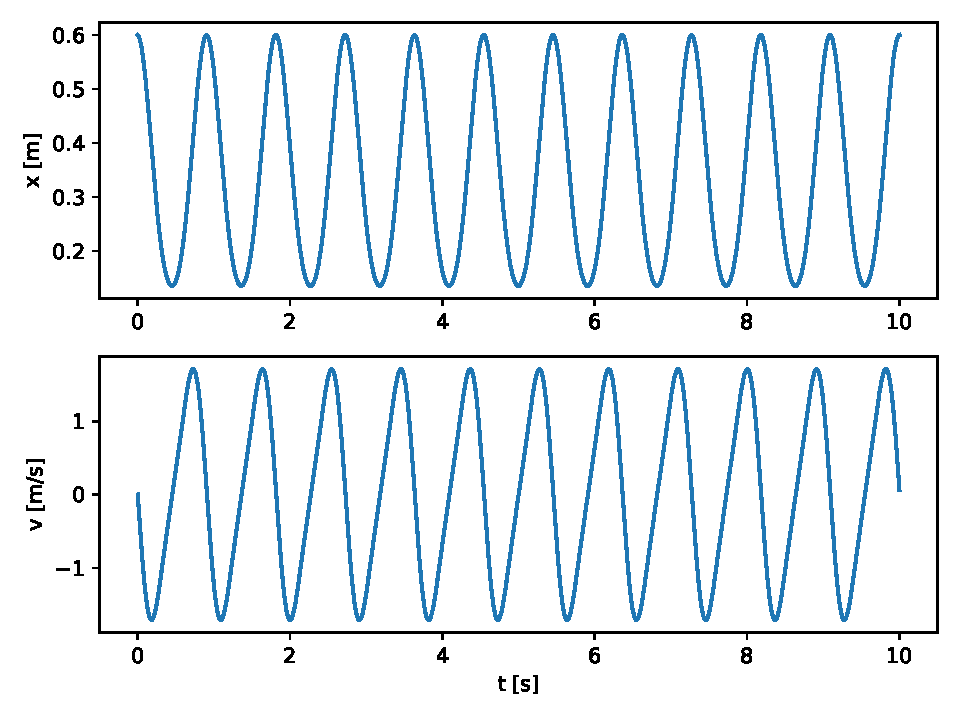
\includegraphics[scale=0.55]{figure_f.pdf}
    \caption{Plot of $x(t), v(t)$ for $t\in[0, 10]$ with $x_1=0.6$m.}
    \label{fig:figure_f}
\end{figure}

The motion is periodic and continuous as expected since there is no friction. We observe that the cylinder oscillates from $x=0.6$m to $x\approx0.1$m.

\section{}
\begin{figure}[h]
    \centering
    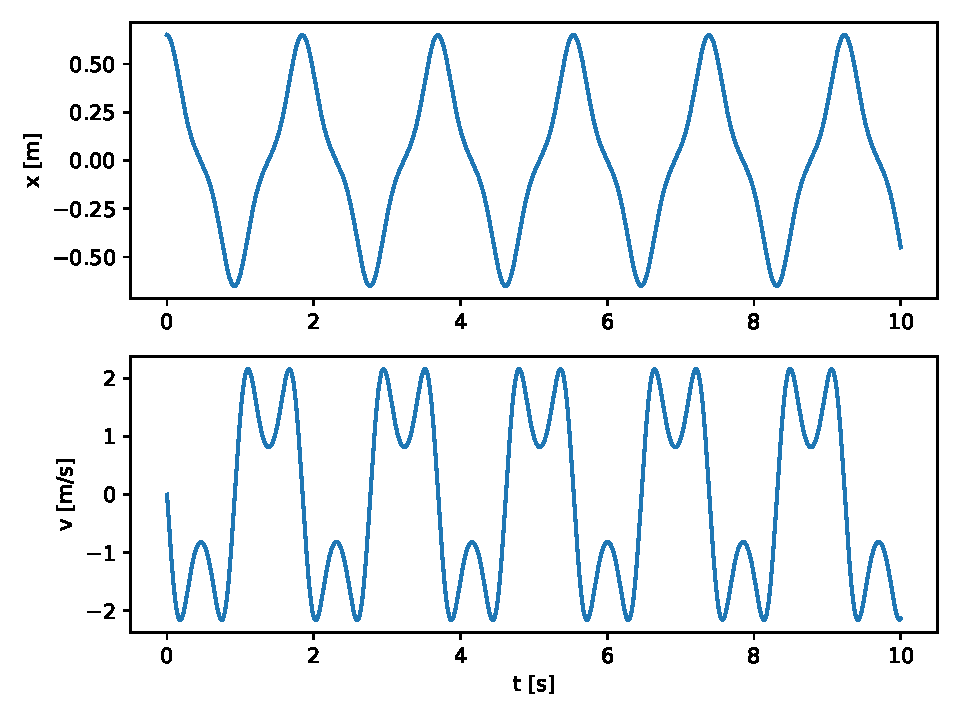
\includegraphics[scale=0.55]{figure_g.pdf}
    \caption{Plot of $x(t), v(t)$ for $t\in[0, 10]$ with $x_1=0.65$m.}
    \label{fig:figure_g}
\end{figure}
With a slight alteration in $x_1$, the cylinder now oscillates between $\pm 0.65$m. When $x=\pm l_0$, will there be zero potential energy stored in the spring as the system is at equilibrium. This means that the kinetic energy has to be at a maximum. We observe two such maximas per period since we have two equilibrium points ($x=\pm0.4$m, seen in Figure \ref{fig:oppgave_e}).

\section{}
The vertical component of $F_k$ is
\begin{align*}
    F_y
    &= F_k \sin\alpha \\
    &= F_k \frac{h}{l_0} \\
    &= -k \frac{h}{l} \sqrt{x^2+h^2}
        \left( 
            1 - \frac{l_0}{\sqrt{x^2+h^2}}
        \right) \\
    &= -k h
        \left( 
            1 - \frac{l_0}{\sqrt{x^2+h^2}}
        \right)
\end{align*}

\section{}
We use Newton's second law in the $y$-direction:
\begin{align*}
    \sum F_y &= 0 \\
    \sum F_y &= N+G+F_y = 0 \\
    N &= -G-F_y = mg + k h
        \left( 
            1 - \frac{l_0}{\sqrt{x^2+h^2}}
        \right)
\end{align*}
When $l=l_0$ the normal force is $N=mg$.

\section{}
For $l<l_0$, the normal force points downwards. Else it points upwards.

\newpage
\section{}
Friction is implemented in the code in section f. We have to take \verb|abs(N)| since the friction force does not depend on the direction of the normal force, only its size, as well as the direction of motion.

\begin{figure}[h]
    \centering
    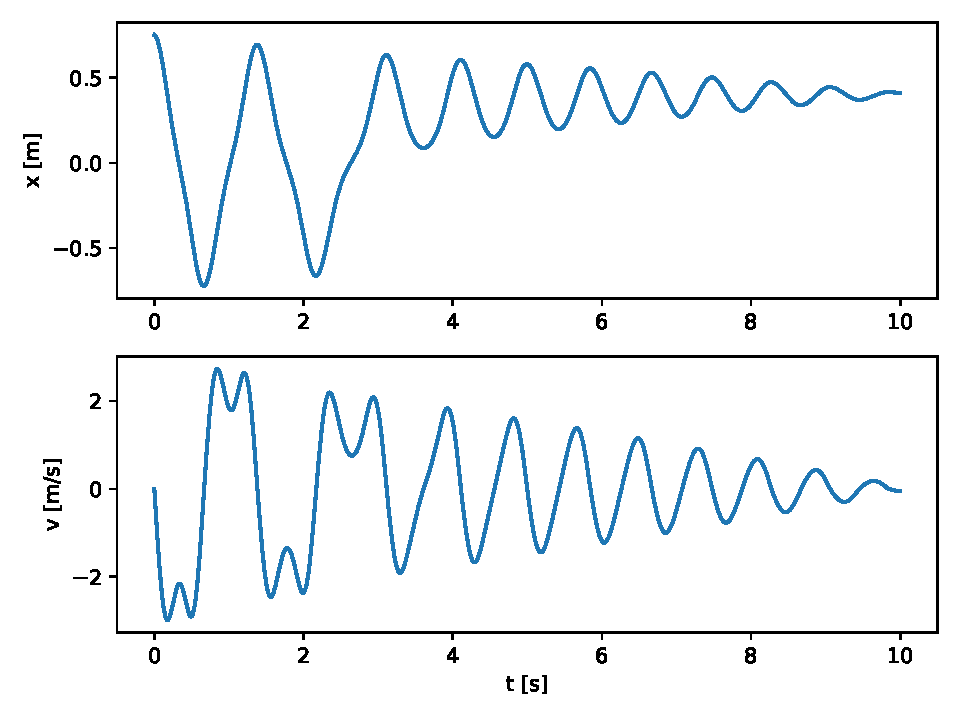
\includegraphics[scale=0.7]{figure_k.pdf}
    \caption{Plot of $x(t), v(t)$ for $t\in[0, 10]$ with $x_1=0.75, \mu=0.05$.}
    \label{fig:figure_k}
\end{figure}
The motion  starts as it did in Figure \ref{fig:figure_g}. After around 3 seconds, the movement is as in Figure \ref{fig:figure_f}, but the motion stops due to the friction.

\newpage
\section{}
\begin{figure}[h!]
    \centering
    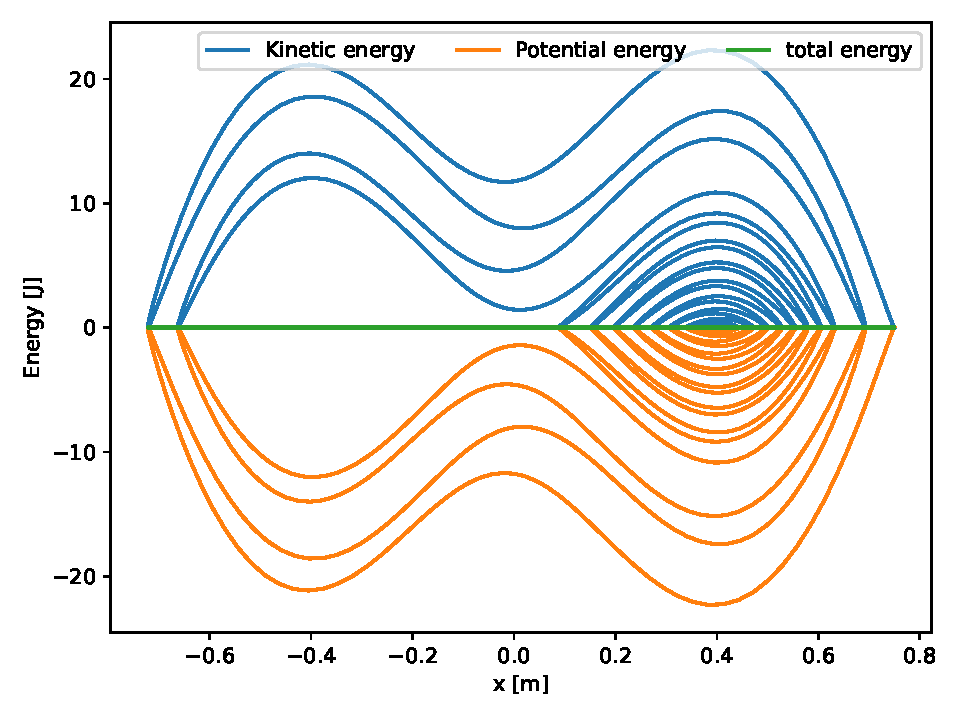
\includegraphics[scale=0.7]{figure_l.pdf}
    \caption{Energy plot for $t\in[0, 10], x_1=0.75, \mu=0.05$.}
    \label{fig:figure_l}
\end{figure}
The energy plot is as expected when compared to Figure \ref{fig:figure_k}. We see the larger oscillations at the start before the cylinders movement changes to smaller oscillations with $x>0$. It eventually stops at the equilibrium point.

\section{}
As mentioned earlier, the system has three equilibrium points: $x=-0.4$, $x=0$, $x=0.4$. As the potential is at a minimum at $x=0$, this is an unstable equilibrium point. At $x=\pm 0.4$, the potential is at its max, making these points stable equilibrium points. 


\end{document}
